
%%%%%%%%%%%%%%%%%%%%%%%%%%%%%%%%% LLM %%%%%%%%%%%%%%%%%%
\begin{frame}{Large Language Models}
   \begin{columns}
         
    %%%%%%%%%%%%%%%%%%%%%%%%%% COLONNE DE GAUCHE %%%%%%%%%%%%%%
       \begin{column}[t]{0.45\textwidth} 
       \begin{block}{Point clés}
           \begin{itemize}
               \item Etat de l'art pour le traitement de language naturel.
               \item Réseaux de Neurones avec une architecture basée sur le  transformer\footnote{Vaswani et al, Attention is all you need,2017 } (annexe \ref{ap:llm_architecture})
               \item Taille : entre 1 et 405 Milliards de neurones
           \end{itemize}
               
       \end{block}
       \end{column}
           
    %%%%%%%%%%%%%%%%%%%%%%%%% COLONNE DE DROITE %%%%%%%%%%%%%%
       \begin{column}[t]{0.5\textwidth}
       \begin{block}{Auto-attention}
           \begin{figure}
               \centering
               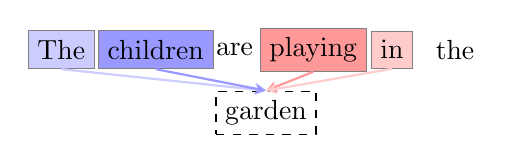
\begin{tikzpicture}[node distance=0.8cm]

    % Define block styles
    \tikzstyle{model} = [rectangle,rounded corners, minimum width=2cm, minimum height=1cm, text centered, draw=black, fill=blue!30]
    \tikzstyle{arrow} = [thick,->,>=stealth]
    
    % Define nodes
    \node (the) [fill=blue!20,rectangle,draw=black!50] {The};
    \node (children) [right of = the,fill=blue!40,rectangle,draw=black!50,xshift=0.4cm] {children};
    \node (are) [right of = children,xshift=0.2cm] {are};
    \node (playing) [right of = are,fill=red!40,rectangle,draw=black!50,xshift=0.2cm] {playing};
    \node (in) [right of = playing,fill=red!20,rectangle,draw=black!50,xshift=0.2cm] {in};
    \node (the2) [right of = in] {the};
    
    \node (garden) [below of = are, xshift=0.4cm,rectangle,dashed,draw=black] {garden};
    
    % Draw arrows
    \draw [arrow,draw=blue!20] (the.south) -- (garden.north);
    \draw [arrow,draw=blue!40] (children.south) -- (garden.north);
    \draw [arrow,draw=red!40] (playing.south) -- (garden.north);
    \draw [arrow,draw=red!20] (in.south) -- (garden.north);
    
    % Add a rectangle around the last four nodes
    \end{tikzpicture}
               \caption{Illustration du mécanisme d'auto-attention}
           \end{figure}    
           L'auto-attention est la clé du LLM, en permettant de comprendre le contexte
       \end{block}  
       \end{column}
            
   \end{columns}
   \end{frame}


%%%%%%%%%%%%%%%%%%%%%%%%%%%%%%%%% Fine Tuning %%%%%%%%%%%%%%%%%%
\begin{frame}{Fine Tuning}
    \begin{table}[h!]
        \centering
        \begin{tabular}{|c|c|c|}
            \hline
            \textbf{Aspect} & \textbf{Pre-entrainement} & \textbf{Fine Tuning} \\
            \hline
            Objectif & Apprentissage général & Adaptation à un domaine \\
            \hline
            Données & Larges et diverses & Restreintes et Spécifiques \\
            \hline
            Ressources & Centaines de GPU & au moins 1 GPU \\
            \hline
            Durée & Semaine/Mois & Heures/Jours \\
            \hline
        \end{tabular}
        \caption{Comparaison entre le Pre-entrainement et le Fine Tuning de LLM}
        \label{tab:pretrain_vs_finetune}
    \end{table}

    \begin{block}{Parameter-Efficient Fine-Tuning (PEFT)}
        \begin{itemize}
            \item Ensemble de méthodes pour réduire le nombre de paramètres à entrainer
            \item Utilisation de la méthode LoRA (annexe \ref{ap:lora})
            \item Amène des nouveaux hyperparamètres
        \end{itemize}
        
    \end{block}
\end{frame}

%%%%%%%%%%%%%%%%%%%%%%%%%%%%%%%%% HPO %%%%%%%%%%%%%%%%%%
\begin{frame}{Optimisation des Hyperparamètres (OHP)}
   \begin{columns}
         
    %%%%%%%%%%%%%%%%%%%%%%%%%% COLONNE DE GAUCHE %%%%%%%%%%%%%%
       \begin{column}[t]{0.3\textwidth} 
       \begin{block}{Hyperparamètres}
         Paramètres qui ne sont pas entrainés par le modèle (learning rate, dropout ...)           
       \end{block}
       \begin{block}{Objectifs}
        \begin{itemize}
            \item Meilleur performance qu'en manuel
            \item Retirer le besoin d'expertise
        \end{itemize}
        
       \end{block}

       \end{column}
           
    %%%%%%%%%%%%%%%%%%%%%%%%% COLONNE DE DROITE %%%%%%%%%%%%%%
       \begin{column}[t]{0.8\textwidth}
        \begin{figure}
            \centering
            \newcommand{\Dtrain}{\mathcal{D}_{train}}
\newcommand{\Dval}{\mathcal{D}_{val}}
\newcommand{\model}{\mathcal{M}}

\begin{tikzpicture}
    \tikzstyle{data}=[rectangle split, rectangle split parts = 2,draw,text centered, fill=yellow!20]
    \tikzstyle{data2}=[draw,text centered, fill=yellow!20]
    \tikzstyle{model} = [rectangle, draw, text centered, fill = blue!20]
    \tikzstyle{function} = [rectangle, draw, text centered, fill = red!20, font = \bfseries]
    \tikzstyle{metrics} = [rectangle, text centered, draw, fill=teal!20]
    
\tikzstyle{dot_arrow} = [thick,dotted,->,>=stealth]

\node (train_data) [data2, align = center]{Données \\ d'entrainement};  

\node (PT_model)[model, below of = train_data,align = center, xshift = 0.1cm]{Modèle \\ Pré-entrainé };

\node (training) [function, right of = PT_model, anchor = west, xshift = 0.35cm]{Fine-Tuning};

\node (hp) [metrics, above of = training]{Hyperparamètres};

\node (FT_model) [model, right of = training, anchor = west, xshift = 0.55cm, align = center]{Modèle \\fine tuné};

\node (val_data) [data2,above of = FT_model, align = center]{Données \\ de validation}; 
        
\node (evaluate) [function, right of = FT_model, anchor = west, xshift = 0.1cm]{Evaluation};

\node (metrics) [metrics, right of = evaluate, anchor = west, xshift = 0.1cm]{résultats};


\begin{scope}[on background layer]
    \node(bbfunction)[draw, thick,fill=black!10,opacity=0.5,draw=black!70, dashed, rounded corners, fit=(train_data) (PT_model) (training) (FT_model)(val_data)(evaluate)(metrics), inner sep=0.1cm, label=155:{Fonction boite noire}] {};
\end{scope}

\draw [dot_arrow] (train_data) -- (training);
\draw [dot_arrow] (PT_model) -- (training);
\draw [dot_arrow] (hp) -- (training);
\draw [dot_arrow] ([xshift = -1.57cm]bbfunction.north) -- (hp.north);
\draw [dot_arrow] (training) -- (FT_model);
\draw [dot_arrow] (val_data) -- (evaluate);
\draw [dot_arrow] (FT_model) -- (evaluate);
\draw [dot_arrow] (evaluate) -- (metrics);
\draw [dot_arrow] (metrics) -- ([xshift = 4.45cm]bbfunction.north);

\node (hpo) [circle, above of = bbfunction, yshift = 0.8cm,xshift=1.415cm,align=center, draw, fill = teal!40]{Opt. \\ Algo.};
\node [left of = hpo, yshift = 0.cm, anchor = south east]{Solution};
\node [right of = hpo, yshift = 0cm,anchor = south west, align = center]{Résultat sur le jeu\\ de validation};

%\draw [thick,->,>=stealth]    ([xshift = 6.25cm]bbfunction.north) to[out=90,in=-5] (hpo.east);
\draw [thick,<-,>=stealth]     (hpo.east)to[out=0,in=90] ([xshift = 4.45cm]bbfunction.north);
\draw [thick,->,>=stealth]     (hpo.west) to[out=180,in=90] ([xshift = -1.57cm]bbfunction.north);




\end{tikzpicture}
            \caption{Fonctionnement général de l'optimisation des hyperparamètres}
       \end{figure}  
       \end{column}
            
   \end{columns}

   

\end{frame}


%%%%%%%%%%%%%%%%%%%%%%%%%%%%%%%%% Formulation PBM %%%%%%%%%%%%%%%%%%
\begin{frame}{Formulation du problème}
    \begin{block}{Equation}
        \begin{equation}
            \eta^* \in \arg \max_{\eta \in \mathcal A}f(\eta), \quad f:\mathbb{R}^d \rightarrow \mathbb{R}
        \end{equation}
        Avec $\eta$ une solution de dimension $d$ et $f$ la fonction représentant l'entrainement et l'évaluation d'un modèle.
    \end{block}

    \begin{block}{Charactéristiques de la fonction $f$}
        \begin{itemize}
            \item Boite-noire : non dérivable
            \item Couteux : une évaluation se compte en dizaine de minutes
            \item Bruité : évaluer 2 fois la même solution peut donner un résultat différent
            \item Variables mixes : les variables sont de plusieurs types (entier, continu...)
        \end{itemize}
        
    \end{block}
    
   
\end{frame}